\PassOptionsToPackage{unicode,pdfusetitle}{hyperref}
\PassOptionsToPackage{hyphens}{url}
\PassOptionsToPackage{dvipsnames,svgnames,x11names}{xcolor}

\documentclass[twoside]{article}

\usepackage[]{aistats2023}
% If your paper is accepted, change the options for the package
% aistats2023 as follows:
%
%\usepackage[accepted]{aistats2023}
%
% This option will print headings for the title of your paper and
% headings for the authors names, plus a copyright note at the end of
% the first column of the first page.

% If you set papersize explicitly, activate the following three lines:
%\special{papersize = 8.5in, 11in}
%\setlength{\pdfpageheight}{11in}
%\setlength{\pdfpagewidth}{8.5in}

% If you use natbib package, activate the following three lines:
%\usepackage[round]{natbib}
%\renewcommand{\bibname}{References}
%\renewcommand{\bibsection}{\subsubsection*{\bibname}}

% If you use BibTeX in apalike style, activate the following line:
%\bibliographystyle{apalike}



%%%%%%%%%%%%%%%%% OUR PREAMBLE  %%%%%%%%%%%%%%%%

\usepackage{lmodern}
\usepackage{amssymb,amsmath,amsthm,mathtools,isomath}

\usepackage[T1]{fontenc}
\usepackage[utf8]{inputenc}
\usepackage{textcomp} % provide euro and other symbols
\usepackage[english]{babel}

\usepackage{upquote} % straight quotes in verbatim environments
\usepackage{nicefrac}	% compact symbols for 1/2, etc.
\usepackage[]{microtype}
\UseMicrotypeSet[protrusion]{basicmath} % disable protrusion for tt fonts

\usepackage{stmaryrd}
\usepackage{xcolor}
\usepackage{xurl}
\usepackage{bookmark}
\usepackage{csquotes}
\usepackage{siunitx}
\usepackage{enumitem}

\usepackage{algorithm,algpseudocode}
\usepackage[titlenumbered,linesnumbered,ruled,noend,algo2e]{algorithm2e}

\usepackage[textsize=scriptsize]{todonotes}
\newcommand{\jonas}[1]{\textcolor{red!20}{[JW: #1]}}
\newcommand{\jw}[1]{\todo[inline,color=red!20]{{\bf JW:} #1}}
\newcommand{\mm}[1]{\todo[inline,color=purple!20]{{\bf Mathurin:} #1}}
\newcommand{\mathurin}[1]{\todo[inline,color=purple!20]{{\bf Mathurin:} #1}}
\newcommand{\klopfe}[1]{\todo[inline,color=orange]{{\bf Klopfe:} #1}}
\newcommand{\qk}[1]{\todo[inline,color=orange]{{\bf Klopfe:} #1}}
\newcommand{\johan}[1]{\todo[inline,color=black!30]{{\bf JL:} #1}}
\newcommand{\jl}[1]{\todo[inline,color=black!30]{{\bf JL:} #1}}
\newcommand{\JL}[1]{{\todo[inline,color=black!30]{{\bf JL:} #1}}}

\newcommand{\widebar}[1]{\mkern 1.5mu\overline{\mkern-1.5mu#1\mkern-1.5mu}\mkern 1.5mu}

\usepackage[noabbrev,nameinlink]{cleveref}

%%%% problem environment
\usepackage{aliascnt}
\newaliascnt{problem}{equation}
\aliascntresetthe{problem}
\creflabelformat{problem}{#2\textup{(#1)}#3}
\makeatletter
\def\problem{$$\refstepcounter{problem}}
\def\endproblem{\eqno \hbox{\@eqnnum}$$\@ignoretrue}
\makeatother
\Crefname{problem}{Problem}{Problems}
%%%%%%%%%%%%%%%%%

\usepackage{hyperref}
\hypersetup{
  colorlinks = true,
  linkcolor  = RoyalBlue4,
  filecolor  = RoyalBlue4,
  citecolor  = VioletRed4,
  urlcolor   = RoyalBlue4
}

\usepackage{longtable}
\usepackage{booktabs}

\usepackage{etoolbox}

% Allow footnotes in longtable head/foot
\usepackage{footnotehyper}
\makesavenoteenv{longtable}

\usepackage{graphicx}
\graphicspath{{../figures/}}
\usepackage{subcaption}

% bibliography
\usepackage[style=authoryear,language=english,uniquelist=false]{biblatex}
\addbibresource{slopecd.bib}

\setlength{\emergencystretch}{3em} % prevent overfull lines

% operators
\DeclareMathOperator*{\argmax}{arg\,max}
\DeclareMathOperator*{\argmin}{arg\,min}
\DeclareMathOperator{\tr}{tr}
\DeclareMathOperator{\diag}{diag}
\DeclareMathOperator{\range}{range}
\DeclareMathOperator{\nullspace}{null}
\DeclareMathOperator{\rank}{rank}
\DeclareMathOperator{\sign}{sign}
\DeclareMathOperator{\dist}{dist}
\DeclareMathOperator{\prox}{prox}
\DeclareMathOperator{\Span}{span}

% delimiters
\DeclarePairedDelimiter\ceil{\lceil}{\rceil}
\DeclarePairedDelimiter\floor{\lfloor}{\rfloor}

% macros
\newcommand{\abs}[1]{\lvert {#1} \rvert}
\newcommand{\norm}[1]{\lVert {#1} \rVert}
\newcommand{\bbR}{\mathbb{R}}
\newcommand{\cB}{\mathcal{B}}
\newcommand{\cC}{\mathcal{C}}
\newcommand{\cM}{\mathcal{M}}
\newcommand{\pkg}[1]{\textsf{#1}}
\newcommand{\dataset}[1]{\texttt{#1}}

% theorems
\theoremstyle{plain}
\newtheorem{theorem}{Theorem}[section]
\newtheorem{proposition}[theorem]{Proposition}
\newtheorem{lemma}[theorem]{Lemma}
\newtheorem{corollary}[theorem]{Corollary}
\theoremstyle{definition}
\newtheorem{definition}[theorem]{Definition}
\newtheorem{assumption}[theorem]{Assumption}
\theoremstyle{remark}
\newtheorem{remark}[theorem]{Remark}
\newtheorem{example}{Example}

%%%%%%%%%%%%%%%%%%%%%%%%%%%%%%%%%%%%%%%%%%%%%%%%%

\begin{document}

% If your paper is accepted and the title of your paper is very long,
% the style will print as headings an error message. Use the following
% command to supply a shorter title of your paper so that it can be
% used as headings.
%
%\runningtitle{I use this title instead because the last one was very long}

% If your paper is accepted and the number of authors is large, the
% style will print as headings an error message. Use the following
% command to supply a shorter version of the authors names so that
% they can be used as headings (for example, use only the surnames)
%
%\runningauthor{Larsson, Klopfenstein, Massias, Wallin}

\twocolumn[%
  \aistatstitle{Coordinate Descent for Slope}
  \aistatsauthor{Johan Larsson \And Quentin Klopfenstein}
  \aistatsaddress{
    Department of Statistics\\
    Lund University\\
    \href{mailto:johan.larsson@stat.lu.se}{\url{johan.larsson@stat.lu.se}}
    \And
    Institution 2 
    \href{mailto:x@y}{\url{x@y}}
  }
  % \aistatsauthor{Mathurin Massias \And Jonas Wallin}
  % \aistatsaddress{
  %   Institution 3
  %   \href{mailto:x@y}{\url{x@y}}
  %   \And
  %   Institution 4
  %   \href{mailto:x@y}{\url{x@y}}
  % }
]

\begin{abstract}
  %!TEX root=./main.tex
% Penalized regression is a core element of modern statistical learning.
Among numerous regression methods, the lasso is the most famous estimator allowing for feature selection. %due to its sparsity.  %solution induced by the $\ell_1$ penalty.
One of the many reasons for its wide usage is the speed at which the underlying optimization problem can be solved, state-of-the-art solvers relying on coordinate descent algorithm.
The Sorted L-One Penalized Estimation (SLOPE) is a generalization of the lasso with appealing statistical properties. The method has not yet reached a wide interest. This is in large extent due to slow performance of the available software, which is due to slow solvers of the underlying optimization problem in large dimension.
%Despite having better statistical properties, the Sorted L-One Penalized Estimation (SLOPE), a generalization of the lasso, has not yet reached a wide interest.
%This is mostly due to the time required to solve the underlying optimization problem in large dimension.
We propose a new fast algorithm to solve the SLOPE optimization problem,
% Despite the non-separability of the penalty, we propose a hybrid method
that combines proximal gradient descent steps and proximal coordinate descent ones.
We provide new results on the directional derivatives of the SLOPE penalty function, its related SLOPE thresholding operator and convergence guarantees for our proposed solver.
To highlight the speed of our method, we performed an extensive benchmark based on simulated and real datasets including a large list of competitors.

\end{abstract}

%!TEX root = ./slopecd.tex
\section{Introduction}\label{sec:introduction}
%%%%%%%%%%%%%%%%%%%%%%%%%%%%%%%%%%%%%%%%%%%%%%

For a fixed non-increasing and non-negative sequence \(\lambda\), the
Sorted L-One Penalized Estimation (SLOPE) problem~\cite{bogdan2013,bogdan2015}
is defined as
\begin{equation}
  \label{eq:slope-problem}
  \operatorname{minimize}_{\beta \in \mathbb{R}^p}
  P(\beta) = L(\beta) + J(\beta)
\end{equation}
where we take \(L\) to be smooth and twice differentiable and
\begin{equation}
  \label{eq:sortedl-l1-norm}
  J(\beta) = \sum_{j=1}^p \lambda_j|\beta_{(j)}|
\end{equation}
is the \emph{sorted \(\ell_1\) norm}, defined such that
\[
  |\beta_{(1)}| \geq |\beta_{(2)}| \geq \cdots \geq |\beta_{(p)}|.
\]

\paragraph{Notation}\label{sec:notation}

Let \((i)^{-}\) be the inverse of \((i)\) such that
\(\big((i)^-\big)^- = (i)\). See \cref{tab:permutation-example} for an
example of this operator for a particular \(\beta\).
\begin{table}
  \centering
  \caption{Example of the permutation operator \((i)\) and its inverse
    \((i)^-\)\label{tab:permutation-example}}
  \begin{tabular}{cccc}
    \toprule
    \(i\) & \(\beta_i\) & \((i)\) & \((i)^-\) \\
    \midrule
    1     & 1         & 2              & 3                \\
    2     & -3        & 3              & 1                \\
    3     & 2         & 1              & 2                \\
    \bottomrule
  \end{tabular}
\end{table}
This means that
\[
  J(\beta) = \sum_{j=1}^p \lambda_j |\beta_{(j)}|
  = \sum_{j=1}^p \lambda_{(j)^-}|\beta_j|.
\]
\mathurin{For a fixed $\beta$}, let \(\mathcal{C}_1, \mathcal{C}_2\, \dots, \mathcal{C}_m\) and \(c_1,
c_2, \dots, c_m\) be the indices and coefficients, respectively, for the \(m\)
clusters of $\beta$ such that
\[
  \mathcal{C}_i = \{j : |\beta_j| = c_i\} \quad \text{and} \quad
  c_1 > c_2 > \cdots > c_m \geq 0.
\]
We also let \(\bar{\mathcal{C}}\) note the complement of \(\mathcal{C}\).


%!TEX root = ./slopecd.tex

\section{Theory}\label{sec:theory}
%%%%%%%%%%%%%%%%%%%%%%%%%%%%%%%%%%%%
\subsection{Directional Derivatives}%
\label{sec:directional-derivatives}
%%%%%%%%%%%%%%%%%%%%%%%%%%%%%%%%%%%%

\subsubsection{The Sorted \texorpdfstring{\(\ell_1\)}{l1}
  Norm}

\begin{theorem}
  \label{thm:sl1-directional-derivative}
  Let \(v \in \bbR^p \setminus \{0\}\), \(h_0 \in \big(0, \min_{i,j \in
    \{i : \beta_i \neq 0\}}\big| |\beta_i| - |\beta_j| \big|/\max_k|v_k| \big]\) and
  define \(\sigma\) to be the permutation such that
  \[
    |\beta + h_0v|_{\sigma(1)} \geq |\beta + h_0v |_{\sigma(2)}
    \geq \cdots \geq |\beta + h_0v|_{\sigma(p)}.
  \]
  \mm{I think we need to state that for any \(h \leq h_0\), \(\sigma\) is still a correct reordering for \(\beta + h v\) (that we use at the last line of \eqref{eq:sl1-directional-derivative})}
  The directional derivative for the sorted \(\ell_1\) norm, \(J(\beta)\), is
  \[
    D_v J(\beta) =
    \sum_{i=1}^m \sum_{j \in \mathcal{C}_i} \lambda_j v_{\sigma(j)}\sign(\beta_{\sigma(j)} + h_0v_{\sigma(j)})\]
  \mm{doesn't the definition of \(h_0\) imply that \(\beta_j + h_0 v_j\) has the sign of \(\beta_j\)?}
  \jl{Not when \(\beta = 0\), since then the sign is determined solely by \(v\).}
  where
  \[
    \mathcal{C}_i = \{j : |\beta_j| = c_i\},\qquad
    c_1 > c_2 > \cdots > c_m \geq 0.
  \]
\end{theorem}
\begin{proof}
  The directional derivative for the sorted \(\ell_1\) norm and a direction
  \(v\) with \(\lVert v \rVert = 1\) \mm{is normalization needed?}\jw{No, but I think we should put in the definition of Theorem, as it no limitation?} is
  \begin{equation}
    \label{eq:sl1-directional-derivative}
    \begin{aligned}
      D_v J(\beta) & = \lim_{h \searrow 0} \frac{J(\beta + h v) - J(\beta)}{h}                                                                     \\
                   & = \lim_{h \searrow 0} \frac{\sum_{j=1}^p\lambda_j\big(|\beta + vh|_{\sigma(j)} - |\beta|_{(j)}\big)}{h}                       \\
                   & = \lim_{h \searrow 0}\frac{\sum_i \sum_{j \in \mathcal{C}_i} \lambda_j\big(|\beta + vh|_{\sigma(j)} - |\beta|_{(j)}\big)}{h}. \\
    \end{aligned}
  \end{equation}
  Assume without loss of generality that \(c_m = 0\).
  Then
  \[
    \sum_{j \in \mathcal{C}_m}\frac{\lambda_j \big( |\beta + vh|_{\sigma(j)} - |\beta|_{(j)}\big)}{h}
    = \sum_{j \in \mathcal{C}_m} \lambda_j \sign(\beta + hv)_{\sigma(j)}v_{\sigma(j)}.
  \]
  Next, recall the construction of \(h_0\) and
  observe that \(\sign(\beta_j + hv_j) = \sign(\beta_j)\)
  and \(\sigma(j) = (j)\) for all \(j \notin \mathcal{C}_m\) \mm{here there is an issue for me because, by the clustering effect, \(()\) is not uniquely defined. Since \(v\) allows each component of \(\beta + h v\) to move at different speed, we may, inside each cluster, end up with any arbitrary order (the limit on the magnitude of \(h\) only imposes that values from one cluster don't end up crossing another cluster )}\jw{I don't follow. You have an arbitrary ordering if \(|\beta_i +hv_i|\) and \(|\beta_j +hv_j|\) otherwise the ordering is defined by \(\sigma\) as it determined by \(\beta\) and \(v\)?}
  \mathurin{It's a small detail, but neither \(\sigma\) nor \(()\) are uniquely defined.
    For me the above sentence says that for \(h\) small enough and the non zero clusters, \(\sigma\) does not depend on \(v\). But if you take \(\beta = (0, 10, 10, 20)\) and \(hv = (0, 1, 0, 0)\) or \(hv = (0, 0, 1, 0)\), they don't yield the same \(\sigma\).
    I'm thinking a rigorous formulation is: "\(\sigma\) is a valid reordering for \(\beta\)"}
  whenever \(0 < h < h_0\).
  It follows that
  \[
    \sum_{j \in \mathcal{C}_i} \frac{\lambda_j\big(|\beta + hv|_{\sigma(j)} - |\beta|_{(j)}\big)}{h}
    = \sum_{j \in \mathcal{C}_i} \lambda_j\sign(\beta + vh)_{\sigma(j)}v_{\sigma(j)}.
  \]
  From this, we see that \eqref{eq:sl1-directional-derivative} reduces to
  \[
    \lim_{h \searrow 0} \sum_i \sum_{j \in \mathcal{C}_i} \lambda_j\sign(\beta + vh)_{\sigma(j)}v_{\sigma(j)}
    = \sum_i \sum_{j \in \mathcal{C}_i} \lambda_j\sign(\beta + vh_0)_{\sigma(j)}v_{\sigma(j)}.
  \]
  \mathurin{Is this reformulation equivalent? (provided \(c_m = 0\))}
  \JL{Yes, good point! But we still need \(h_0\) for the permutation.}
  Then it follows that
  \begin{equation*}
    D_v J(\beta) = \sum_{j \notin \cC_m} \lambda_j \sign (\beta_{\sigma(j)}) v_{\sigma(j)}
    +
    \sum_{j \in \cC_m} \lambda_j \sign (v_{\sigma(j)}) v_{\sigma(j)}.
  \end{equation*}
\end{proof}

\begin{remark}
  Using \cref{thm:sl1-directional-derivative}, we see that
  the directional derivative for \eqref{eq:slope-problem} is
  \[
    D_v P(\beta) = v^T \big(\nabla L(\beta)\big) + D_v J(\beta).
  \]
\end{remark}

\subsection{Coordinate Updates}%
\label{sec:coordinate-updates}

We will now consider the variable \(\tilde \beta_k\) which equals the magnitude of the \(k\)th cluster, that is \(|\beta_j|=\tilde \beta_k\) for all \(j \in \mathcal{C}_k\).
We will now derive the method how to update the parameters in the coordinate that corresponds to keeping the clusters fixed, which is equivalent to minimizing \(P(\beta)\) over \(\tilde \beta_k\).
Evaluating the objective function at \(\beta\) we have
\[
  \begin{aligned}
    P(\beta) & =  \frac{1}{2} \lVert y - X\beta\rVert_2^2 + J(\beta)                                                                                                                                                                                                                                       \\
             & = \frac{1}{2} \lVert y - X_{\bar{\mathcal{C}_k}} \beta_{\bar{\mathcal{C}_k}} - \big(X_{\mathcal{C}_k} s_{\mathcal{C}_k}\big)\tilde\beta_k  \rVert_2^2 + \sum_{j \notin {\mathcal{C}_k}} \lambda_{(j)^-}|\beta_k| + \bigg(\sum_{j \in {\mathcal{C}_k}} \lambda_{(j)^-}\bigg)|\tilde\beta_k|,
  \end{aligned}
\]
where \(s=\sign(\beta)\). We can consider this as subproblem trying to minimize the one-dimensional function
\[
  \begin{aligned}
    P(\tilde \beta_k) & = \frac{1}{2} \lVert r_k - \tilde x_k \tilde \beta_k \beta_{\bar{\mathcal{C}_k}} - \big(X_{\mathcal{C}_k} \beta_{\mathcal{C}_k}\big)c_k  \rVert_2^2 + \sum_{j \notin {\mathcal{C}_k}} \lambda_{(j)^-}|\beta_k| + \bigg(\sum_{j \in {\mathcal{C}_k}} \lambda_{(j)^- }\bigg) |\tilde \beta_k|,
  \end{aligned}
\]
where \(\tilde y_k = X_{\bar{\mathcal{C}}_k} \beta_{\bar{\mathcal{C}_k}}\), \( \tilde x_k = X_{\mathcal{C}_k} s_{\mathcal{C}_k}\),
and \(\tilde r_k= y - \tilde y_k\) is the \emph{partial residual}. An alternative formulation (with identical solution) is to minimize
\[
  \begin{aligned}
    P(c_k) & = \frac{1}{2} \lVert y - X_{\bar{\mathcal{C}_k}} \beta_{\bar{\mathcal{C}_k}} - \big(X_{\mathcal{C}_k} \beta_{\mathcal{C}_k}\big)c_k  \rVert_2^2 + \sum_{j \notin {\mathcal{C}_k}} \lambda_{(j)^-}|\beta_k| + |c_k|\bigg(\sum_{j \in {\mathcal{C}_k}} \lambda_{(j)^- }|\beta_j|\bigg),
  \end{aligned}
\]
and \(\beta_k := c_k\beta_k\).
Now take
derivate with respect to \(\tilde\beta_k\), yielding
\begin{equation}
  \label{eq:cluster-grad}
  \partial_{\tilde\beta_k}
  P(\beta) = \tilde r^T \tilde x + \tilde x^T \tilde x \tilde\beta_k + \partial_{\tilde\beta_k}\Bigg(\bigg(\sum_{j \in {\mathcal{C}_k}} \lambda_{(j)^-}\bigg)|\tilde\beta_k| + \sum_{j \notin \mathcal{C}_k}\lambda_{(j)^-}|\beta_j|\Bigg),
\end{equation}
where the last term is the partial subdifferential of the sorted \(\ell_1\)
norm.
The optimality condition for the sub-problem is \(\boldsymbol{0} \in
\partial_{\tilde \beta} P(\beta).
\)
We now derive a closed form expression for the subdifferential
of the sorted \(\ell_1\) norm.
\begin{theorem}
  \label{thm:cluster-subdifferential}
  The partial subdifferential for the sorted \(\ell_1\) norm with respect
  to \(\tilde\beta_k\), is
  \[
    \partial_{\tilde \beta_k}  J(\beta)       =
    \begin{cases}
      \big[-\sum_{j=1}^{|C(0)|}\lambda^{C(0)}_j, \sum_{j=1}^{|C(0)|}\lambda^{C(0)}_j\big]                                                                        & \text{if } \tilde\beta = 0,           \\
      \big[\sum_{j=|\mathcal{C}_i| - |\mathcal{C}_k|+1}^{|\mathcal{C}_i|}\lambda^{\mathcal{C}_i}_j, \sum_{j=1}^{|\mathcal{C}_k|}\lambda^{\mathcal{C}_i}_j\big]   & \text{if } \tilde\beta = c_i \neq 0,  \\
      \big[-\sum_{j=1}^{|\mathcal{C}_k|}\lambda^{\mathcal{C}_i}_j, -\sum_{j=|\mathcal{C}_i| - |\mathcal{C}_k|+1}^{|\mathcal{C}_i|}\lambda^{\mathcal{C}_k}_j\big] & \text{if } \tilde\beta = -c_i \neq 0, \\
      \{\sign(\tilde\beta)\boldsymbol{1}^T\lambda^{C(\tilde\beta)}\}                                                                                             & \text{otherwise.
      }
      % \{\sign(\tilde\beta) S\big(C(\tilde\beta)\big)\}                                                                                                & \text{if } \tilde\beta \neq c_i \neq 0, \\
      % [-S(\mathcal{C}_m), S(\mathcal{C}_m)]                                                                                                           & \text{if } \tilde\beta = 0,             \\
      % [\sign(\tilde\beta)S\big( C(c_i - \sign(\tilde\beta)\varepsilon_i)\big), \sign(\tilde\beta)S\big(C(c_i + \sign(\tilde\beta)\varepsilon_i)\big)] & \text{if } |\tilde\beta| = c_i,
    \end{cases}
  \]
\end{theorem}
\begin{proof}
  Consider a fixed \(\beta\) and set \(\beta_{\mathcal{C}_k}= s_{\mathcal{C}_k}x\).
  Now let us consider the function  \(f(x) = |x|\sum_{j \in \mathcal{C}_k}\lambda^x_{(j)^-} + \sum_{j \notin \mathcal{C}_k} \lambda^x_{(j)^-}|\beta_j|\), where the ordering of \(\lambda^x\) is with respect to the vector
  \[
    \beta(x)_k = \begin{cases}
      |x|       & \text{if } \mbox{\(k \in \mathcal{C}_k\)}, \\
      |\beta_k| & \mbox{otherwise}.
    \end{cases}
  \]
  .\mathurin{If \(f\) is only a function of \(\tilde \beta\), then the second term is constant, and since we are interested in subgradients, we should able to omit it?} \jonas{I added the notation so that it is clear that ordering of the \(\lambda\) depends on \(x\), hence we can not remove the second component.}
  \(g\in \mathbb{R} \) \mm{\(f/g\) > \(u\) or \(v\) for subgradient?} is a subgradient of \(f\) at \(x\) if
  \begin{equation}
    \label{eq:subgrad-ineq}
    f(x^*)=|x^*|\sum_{j \in C_k}\lambda^{x^*}_{(j)^-} + \sum_{j \notin C(x^*)}\lambda ^{x^*}_{(j)^-}|\beta_j|
    \geq f(x)+ g(x^* - x)=|x|\sum_{j \in C_k} \lambda^x_{(j)^-} + \sum_{j \notin C_k}\lambda^x_{(j)^-}|\beta^x_j| + g(x^* - x)
  \end{equation}
  for all \(x^* \in \mathbb{R}\).
  Without loss of generality, since \(f\) is convex \mathurin{here I did not understand the WLOG relationship with convexity}, assume that we have
  a vector \(\beta\) such that there are two clusters: one corresponding
  to \(\tilde\beta\), which we are optimizing over, and
  one additional cluster \(\mathcal{C}_q\) with corresponding
  coefficient \(c_q\).
  Then we can rewrite \eqref{eq:subgrad-ineq} as
  \[
    |y|S\big(C(y)\big) + c_q S\big(\widebar{C(y)}\big) \geq
    |x| S\big(C(x)\big) + c_q S\big(\widebar{C(x)}\big) + g(y - x).
  \]
  First observe that any \(g\) is permissible whenever \(x = y\).

  At \(x = 0\), \eqref{eq:subgrad-ineq} reduces to
  \[
    |y|S\big(C(y)\big) + c_q S\big(\widebar{C(y)}\big)
    \geq c_q S(\mathcal{C}_1) + gy.
  \]
  Because \(f\) is convex, it is sufficient to consider \(|y| < c_q\),
  in which case \(C(y) = \mathcal{C}_1\) and hence
  \begin{equation}
    |y|S(\mathcal{C}_2) + c_q S(\mathcal{C}_1) \geq c_q S(\mathcal{C}_1) + gy \implies
    |y|S(\mathcal{C}_2) \geq gy,
  \end{equation}
  which means that \(-S(\mathcal{C}_2) \leq g \leq S(\mathcal{C}_2)\).

  If \(x = c_q\), \eqref{eq:subgrad-ineq} becomes
  \[
    |y|S\big(C(y)\big) + x S\big(C(x)\big) \geq x(S(\mathcal{C}_1) + S(\mathcal{C}_2)) + g(y - x).
  \]
  For \(y > x\) we have \(C(y) = \mathcal{C}_1\) and consequently
  \[
    y\big(S(\mathcal{C}_1) - g\big) + x\big(g - S(\mathcal{C}_1)\big) \geq 0,
  \]
  which means that \(g \leq S(\mathcal{C}_1)\).
  Then, for \(0 < y < x\), we see
  \[
    y\big(S(\mathcal{C}_2) - g\big) + x(g - S(\mathcal{C}_2)\big) \geq 0,
  \]
  and hence \(g \geq S(\mathcal{C}_2)\).
  Using the same argument for \(x = -c_q\), we find that we in this case
  must have \(g\) such that
  \(-S(\mathcal{C}_1) \geq g \geq - S(\mathcal{C}_2)\).
  For all other choices of \(x\), \(f\) is differentiable with
  derivative \(\sign(\tilde\beta)S\big(C(\tilde\beta)\big)\).
\end{proof}

The objective and subgradient for the cluster-wise problem are shown in
\cref{fig:cluster-grad-obj}.

\begin{figure}[htbp]
  \centering
  \includegraphics[]{clusterupdate-grad-obj}
  \caption{%
    Objective and gradient under the constraint that we have a fixed
    cluster.
    The optimum is found at \(\tilde\beta = 0.3\).
  }%
  \label{fig:cluster-grad-obj}
\end{figure}

Let \(\mathcal{B}\) be a cluster initialized to \(\mathcal{C}_k\), with
corresponding coefficient \(c_k\).
Then the coordinate update for \(\beta_\mathcal{B}\) is\jl{This obviously
  does not work when \(s=0\). Can we just set \(s = 1\) here? It's just
  the relative signs that really matter, right?}\jw{That is a really good point. Do you think we can tie to the sign of the gradient instead?. We also will not move the zero cluster this way suspect. But it should work for any formation then sign of the gradient is the way I think?}
\jl{Yes, I think you're right, in fact that's what I have in the code now.}
\[
  \beta_\mathcal{B} \gets
  s_\mathcal{B}
  T \left(
  \frac{\tilde r^T \tilde x}{\tilde x^T \tilde x},
  \frac{\lambda}{\tilde x^T \tilde x},
  k,
  \tilde \beta,
  \mathcal{C}
  \right)
\]
where

\begin{equation}
  \label{eq:slope-thresholding}
  T(a, \lambda,k,\tilde \beta, \mathcal{C}) =
  \begin{cases}
    0                                                                 & \text{if } |a| \leq \sum_{i=1}^{|\mathcal{C}_k|}\lambda^{C_0}_i                                                                                                                               \\
    \sign(a)|\tilde \beta_i|                                          & \text{if } \sum_{j= |\mathcal{C}_i| - |\mathcal{C}_k| + 1}^{|\mathcal{C}_i|} \lambda^{\mathcal{C}_i}_j \leq |a| - |\tilde \beta_i| \leq \sum_{j=1}^{|\mathcal{C}_k|}\lambda^{\mathcal{C}_i}_j \\
    \sign(a)\big(|a| - \sum_{j \in \mathcal{C}_k}\lambda_{(j)^-}\big) & \text{otherwise.
    }
  \end{cases}
\end{equation}
To emphasize the connection between \(T\) and the soft-thresholding operator
for the lasso, we call this operator the SLOPE-thresholding operator.
In \cref{fig:slope-thresholding}, we visualize the operator.

\begin{figure}[htbp]
  \centering
  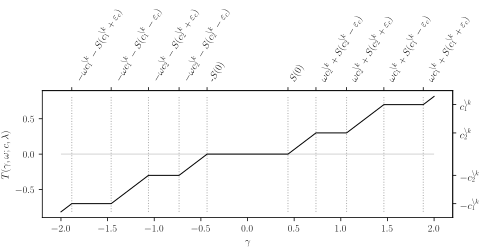
\includegraphics[]{slope-thresholding.pdf}
  \caption{The result of the SLOPE thresholding update.}
  \label{fig:slope-thresholding}
\end{figure}

\subsection{Hybrid proximal coordinate descent strategy}

\begin{algorithm}[tb]
  \SetKwInOut{Init}{init}
  \SetKwInOut{Input}{input}
  \caption{%
    Hybrid coordinate descent and proximal gradient descent algorithm
    for SLOPE\label{alg:hybrid}}
  \Input{
    \(X \in \mathbb{R}^{n\times p}, y\in \mathbb{R}^n, \beta\in \mathbb{R}^p, \lambda \in \{\mathbb{R}^p : \lambda_1 \geq \lambda_2 \geq \cdots > 0\}\), \(m \in \mathbb{N}\)}

  \Init{\(t \gets 0\), \(\beta \gets 0\), \(L \gets \lVert X \rVert_2^2\)}

  \Repeat{convergence}{
  \(t \gets t + 1\)

  \If{\(t \bmod m = 0\)}{

    \(\beta \leftarrow \operatorname{prox}_{J / L}(\beta - \frac{1}{L}\nabla f(\beta))\) \label{alg:hybrid-istastep}

  % \(C_1, \hdots, C_m \leftarrow \mathtt{get\_clusters}(\beta)\)
  }
  \Else{
    \(k \gets 0\)

    \While{\(k \leq \lvert \mathcal{C} \rvert\)}{
      \(k \gets k + 1\)

      \(s \leftarrow \mathrm{sign}(\beta_{\mathcal{C}_k})\)

      \If{\(s \neq 0\)}{
        % \(L_k \gets (X_{:, \mathcal{C}_k}s)^\top  X_{:, \mathcal{C}_k}s\)

        % \(\tilde{\beta} \gets T(|\beta_{\mathcal{C}_k}| - \frac{1}{L_k} \nabla_{\mathcal{C}_k}f(\beta)^\top s, \frac{\lambda}{L_k})\)

        % \(\beta_{\mathcal{C}_k} \leftarrow \tilde{\beta} s\)
        \(\tilde x_k \gets X_{\mathcal{C}_k}s\)

        \(\tilde y_k \gets X_{\widebar{\mathcal{C}}_k}\beta_{\widebar{\mathcal{C}}_k}\)

        \(\tilde r_k \gets y - \tilde y_k\)

        \(
        \beta_{\mathcal{C}_k} \gets
        s T \left(
        \frac{\tilde r^T_k \tilde x_k, }{ \tilde x_k^T \tilde x_k},
        \frac{\lambda}{ \tilde x_k^T \tilde x_k},
        k,
        \tilde \beta,
        \mathcal{C}
        \right)
        \)
        \Comment{\(\mathcal{C}\) is updated at this step.}

      }

    }
  }

  }
  \Return{\(\beta\)}
\end{algorithm}

\begin{theorem}
  Iterates of \cref{alg:hybrid} converge towards \(\beta^*\).
\end{theorem}
\begin{proof}
  First note that convergence properties of proximal gradient descent on convex
  problems such as SLOPE are well-established
  \parencite{beck2009,daubechies2004}, which certifies that updates via
  \cref{alg:hybrid-istastep} make progress towards \(\beta^*\).

  Next note that the objectives of \eqref{eq:slope-problem} and
  \eqref{eq:subproblem} are equal and that \eqref{eq:subproblem} can be seen
  viewed as a version of \eqref{eq:slope-problem} with added linear constraints
  that is also convex. And, finally, because the coordinate updates of
  \cref{alg:hybrid} minimize the sub-problem, we in the worst case make no
  progress and therefore have guaranteed converge rate no less than \(1/m\)
  of that of proximal gradient descent.
\end{proof}


\section{Experiments}\label{sec:experiments}
%%%%%%%%%%%%%%%%%%%%%%%%%%%%%%%%%%%%%%%%%%%

The proposed algorithm is part of a python package relying on numpy and numba~\parencite{harris2020,lam2015}.
It will be made open-source upon publication. To compare its efficiency, we used several public datasets described in \cref{table:datasets}.
We performed an extensive benchmark with the following competitors:
\begin{itemize}[noitemsep]
  \item Alternating Direction Method of Multipliers (\texttt{admm})~\parencite{boyd2010}
  \item Anderson acceleration for proximal gradient descent (\texttt{anderson})~\parencite{zhang2020}
  \item Proximal Gradient Descent (\texttt{pgd})~\cite{combettes2005}
  \item Fast Iterative Shrinkage-Thresholding Algorithm (\texttt{fista})~\parencite{beck2009}
  \item Semismooth Newton-Based Augmented Lagrangian (\texttt{newt-alt})~\parencite{Ziyan2019}
  \item The Oracle solver (\texttt{oracle}) uses the clusters obtained via another
        solver to compute coordinate descent updates from the known solver.
  \item The Hybrid (ours) (\texttt{hybrid}) solver (see \cref{alg:hybrid}) combines proximal gradient descent
        and coordinate descent to overcome the non-separability of the SLOPE problem.
\end{itemize}

\begin{table}[]
  \centering
  \label{table:datasets}
  \begin{tabular}{
      l
      S[table-format=6.0,round-mode=off]
      S[table-format=7.0,round-mode=off]
      S[table-format=1.4,round-mode=off]
      c
    }
    \toprule
    Datasets    & \(n\) & \(p\)   & {Density} \\ \midrule
    Simulated 1 & 200   & 20000   & 1         \\
    Simulated 2 & 20000 & 200     & 1         \\
    Simulated 3 & 200   & 2000000 & 0.001     \\
    Rhee2006    & 842   & 361     & ?         \\
    bcTCGA      & 536   & 17322   & 1         \\
    Scheetz2006 & 120   & 18975   & ?         \\ \bottomrule
  \end{tabular}
\end{table}

We used the \texttt{benchopt}~\parencite{moreau2022benchopt} tool to obtain the convergence curves for the different solvers.
\texttt{Benchopt} launches each solver several times increasing the number of iterations and store the objective value, dual gap and time to reach it.
The repository to reproduce the benchmark is available at XXX.

\subsection{Simulated data}

The design matrix $X$ is simulated with correlation between features $j$ and $j'$ equal to $\rho^{|j-j'|}$ where $\rho$ is a parameter that can be chosen in $[0, 1[$.
The true regression vector $\beta^\star$ contains a certain number of non-zero entries that are obtained by simulating a gaussian distribution with zero mean and unit variance.
The observations are equal to $y=X\beta^\star + \varepsilon$ where $\varepsilon$ is a centered gaussian distribution with variance such that $\lVert X\beta^\star\rVert / \lVert \varepsilon \rVert = 3$.

\subsection{Real data}
\klopfe{Do we keep the three different values for $q$ that changes the sequence of lambas?}
\begin{figure*}[htb]
  \centering
  \includegraphics[scale=0.47]{Rhee2006_legend.pdf}
  \includegraphics[scale=0.5]{Rhee2006.pdf}
  \caption{Benchmark on the Rhee2006 dataset.}
  \label{fig:Rhee2006}
\end{figure*}

\section{DISCUSSION}\label{sec:discussion}
%%%%%%%%%%%%%%%%%%%%%%%%%%%%%%%%%%%%%%%%%

In this paper we have presented a new, fast algorithm for solving Sorted L-One Penalized Estimation (SLOPE).
Our method relies on a combination of proximal gradient descent steps that split clusters and coordinate descent steps that optimize a subproblem, which together guarantee fast convergence.
In our results, we have shown that our method outperforms all competitors for a large variation of real and simulated datasets.

We have not, in this paper, considered using screening rules for SLOPE~\parencite{larsson2020c,elvira2022}.
Although screening rules work for any algorithm considered in this article, they are particularly effective when used in tandem with coordinate descent~\parencite{fercoq2015} and, in addition, easy to implement due to the nature of coordinate descent steps.
This point also holds to when fitting a path of \(\lambda\) sequences~\parencite{friedman2007,friedman2010}, which is often used during cross-validation to obtain an optimal \(\lambda\) sequence. 

Future research may consider alternative strategies to split clusters, for instance batch stochastic gradient descent, which should reduce the burden of the cluster splitting step.

% \subsubsection*{Acknowledgements}

The experiments presented in this paper were carried out using the HPC facilities of the University of Luxembourg~\parencite{Varette2022} (see \texttt{\href{http://hpc.uni.lu}{hpc.uni.lu}}).

The results shown here are in whole or part based upon data generated by the TCGA Research Network: \url{https://www.cancer.gov/tcga}.


\clearpage % do we need this?
\printbibliography[heading=subbibliography]

\onecolumn

\appendix

\aistatstitle{Supplement to \emph{Coordinate Descent for SLOPE}}

\section{Proofs}\label{sec:proofs}

\subsection{Proof of \Cref{thm:sl1-directional-derivative}}

\begin{proof}
  By the definition of the directional derivative,
  \begin{align}
    \phi'(z; \delta)
    = & \lim_{h \downarrow 0} \frac{\phi(z + h \delta) - \phi(z)}{h} \nonumber \\
    = &
    \lim_{h \downarrow 0} \frac{1}{h}
    \left(
      |z + h \delta| \smashoperator{\sum_{j \in C(z + h \delta)}} \lambda_{(j)^-_{z + h \delta}}
      + \smashoperator{\sum_{j \notin C(z + h\delta)}} |\beta_j| \lambda_{(j)^-_{z + h \delta}}
      - |z| \smashoperator{\sum_{j \in C(z)}} \lambda_{(j)^-_z}
      - \smashoperator{\sum_{j \notin C(z)}} |\beta_j| \lambda_{(j)^-_z}
    \right) \nonumber                                                          \\
    = & \lim_{h \downarrow 0}
    \frac{1}{h}
    \left(
      |z + h \delta| \smashoperator{\sum_{j \in C(z + {\varepsilon_c}\delta)}} \lambda_{(j)^-_{z + {\varepsilon_c}\delta}}
      + \smashoperator{\sum_{j \notin C(z + {\varepsilon_c}\delta)}} |\beta_j| \lambda_{(j)^-_{z + {\varepsilon_c}\delta}}
      - |z| \smashoperator{\sum_{j \in C(z)}} \lambda_{(j)^-_{z}}
      - \smashoperator{\sum_{j \notin C(z)}} |\beta_j| \lambda_{(j)^-_{z}}
    \right)
    \label{eq:directional-derivative-sl1}
  \end{align}
  We have the following cases to consider: \(|z| \in c^{(k)}\),
  \(|z| = 0\), and \(|z| \notin \{0\} \cup c^{(k)}\).

  Starting with\(|z| = c_i^{(k)}\), note that we have,
  as a result of the definition of
  \({\varepsilon_c}\), the following identities:
  \begin{align*}
    C(c_i^{(k)} + {\varepsilon_c}\delta)            & \subseteq C(c_i^{(k)}),                                                                                                                                 \\
    \tilde{\mathcal{C}}_i                           & = \widebar{C(c_i^{(k)} + {\varepsilon_c} \delta)} \cap C(c_i^{(k)}),                                                                                    \\
    C(c_i^{(k)})                                    & = \tilde{C}_i \cup \big(C(c_i^{(k)} + {\varepsilon_c}\delta) \cap C(c_i^{(k)})\big) = \tilde{\mathcal{C}}_i \cup C(c_i^{(k)} + {\varepsilon_c} \delta), \\
    \widebar{C(c_i^{(k)} + {\varepsilon_c} \delta)} & = \widebar{C(c_i^{(k)})} \cup \tilde{\mathcal{C}}_i.
  \end{align*}
  Using this, we can rewrite \eqref{eq:directional-derivative-sl1} as
  \begin{equation*}
    \label{eq:directional-derivative-simplified}
    J'_k(z; \delta)
    = \lim_{h \downarrow 0} \frac{1}{h}
    \left(
      \splitfrac{
      |z + h\delta|\smashoperator{\sum_{j \in C(z + {\varepsilon_c}\delta)}} \lambda_{(j)^-_{z + {\varepsilon_c}\delta}}
      + |c_i^{(k)}|\smashoperator{\sum_{j \in \tilde{C}_i}} \lambda_{(j)^-_{z + {\varepsilon_c}\delta}}
      + \smashoperator{\sum_{j \in \widebar{C(z)}}} |\beta_j|\lambda_{(j)^-_{z + {\varepsilon_c}\delta}}
      }{%
      - |z| \smashoperator{\sum_{j \in \tilde{\mathcal{C}}_i}} \lambda_{(j)^-_{z}}
      - |c_i^{(k)}| \smashoperator{\sum_{j \in C(z + {\varepsilon_c}\delta)}} \lambda_{(j)^-_{z}}
      - \smashoperator{\sum_{j \in \widebar{C(z)}}} |\beta_j| \lambda_{(j)^-_{z}}
      }
    \right).
  \end{equation*}
  Next, observe that \(\lambda_{(j)^-_{z + {\varepsilon_c}\delta}} =
  \lambda_{(j)^-_{z}}\) for all \(j \in \widebar{C(z)}\) and consequently
  \[
    \smashoperator{\sum_{j \in \widebar{C(z)}}} |\beta_j|\lambda_{(j)^-_{z + {\varepsilon_c}\delta}} =
    \smashoperator{\sum_{j \in \widebar{C(z)}}} |\beta_j|\lambda_{(j)^-_{z}}.
  \]
  Moreover, note that, since \(z = \pm c_i\), there exists a permutation corresponding to
  \(\lambda_{(j)^-_{z}}\) such that
  \[
    |z|\smashoperator{\sum_{j \in \tilde{C}_i}} \lambda_{(j)^-_{z + {\varepsilon_c}\delta}}
    = |c^{(k)}_i| \smashoperator{\sum_{j \in \tilde{C}_i}} \lambda_{(j)^-_{z}}
  \]
  and consequently
  \begin{equation}
    \label{eq:directional-derivative-simplified-again}
    J'_k(z; \delta)
    = \lim_{h \downarrow 0} \frac{1}{h}
    \left(
      |z + h\delta|\smashoperator{\sum_{j \in C(z + {\varepsilon_c}\delta)}} \lambda_{(j)^-_{z + {\varepsilon_c}\delta}}
      - |c_i^{(k)}| \smashoperator{\sum_{j \in C(z + {\varepsilon_c}\delta)}} \lambda_{(j)^-_{z}}.
    \right).
  \end{equation}
  Now, since \(c_i^{(k)} + h \delta > 0\) and \(-c_i^{(k)} + h \delta < 0\) in the limit as
  \(h\) goes to \(0\) for \(c_i \neq 0\), we have
  \[
    \lim_{h\downarrow 0} |-c_i + h \delta|
    = \lim_{h\downarrow 0}\big( |c_i^{(k)}| -h \delta\big)
    \quad\text{and}\quad
    \lim_{h\downarrow 0} |c_i^{(k)} + h \delta|
    = \lim_{h\downarrow 0}(|c_i^{(k)}| + h \delta)
  \]
  which means that
  \begin{align*}
    J'_k(z; \delta)
     & = \lim_{h \downarrow 0} \frac{1}{h}
    \left(
      \big(|z| + \sign(z)h\delta\big)\smashoperator{\sum_{j \in C(z + {\varepsilon_c}\delta)}} \lambda_{(j)^-_{z + {\varepsilon_c}\delta}}
      - |c_i| \smashoperator{\sum_{j \in C(z + {\varepsilon_c}\delta)}} \lambda_{(j)^-_{z}}.
    \right)                                                                                                                  \\
     & = \lim_{h \downarrow 0} \frac{1}{h}
    \sign(z)h\delta\smashoperator{\sum_{j \in C(z + {\varepsilon_c}\delta)}} \lambda_{(j)^-_{z + {\varepsilon_c}\delta}}     \\
     & = \sign(z)\delta\smashoperator{\sum_{j \in C(z + {\varepsilon_c}\delta)}} \lambda_{(j)^-_{z + {\varepsilon_c}\delta}} \\
  \end{align*}

  For the case when \(z=0\) there are two sub-cases to consider. First, when \(c_m^{(k)} = 0\) then
  \eqref{eq:directional-derivative-simplified-again} is simply
  \begin{equation*}
    \label{eq:directional-derivative-zerocase}
    J'_k(0; \delta)
    = \lim_{h \downarrow 0} \frac{1}{h}
    |h\delta|\smashoperator{\sum_{j \in C({\varepsilon_c}\delta)}} \lambda_{(j)^-_{{\varepsilon_c}\delta}}
    = \smashoperator{\sum_{j \in C({\varepsilon_c}\delta)}} \lambda_{(j)^-_{{\varepsilon_c}\delta}}
  \end{equation*}
  since \(|\delta| = 1\) by definition.

  The other sub-case is \(c_m^{(k)} \neq 0\). Here
  \eqref{eq:directional-derivative-sl1} reduces to
  \begin{equation*}
    J_k'(0; \delta) = \lim_{h \downarrow 0}
    \frac{1}{h}
    \left(
      |h \delta| \smashoperator{\sum_{j \in C({\varepsilon_c}\delta)}} \lambda_{(j)^-_{{\varepsilon_c}\delta}}
      + \smashoperator{\sum_{j \notin C({\varepsilon_c}\delta)}} |\beta_j| \lambda_{(j)^-_{{\varepsilon_c}\delta}}
      - \smashoperator{\sum_{j \notin C(0)}} |\beta_j| \lambda_{(j)^-_{0}}
    \right).
  \end{equation*}
  In this case, we have \(C(0) = C({\varepsilon_c}\delta)\) since \(c_m^{(k)}
  \neq 0\), and therefore
  \[
    \smashoperator{\sum_{j \notin C({\varepsilon_c}\delta)}} |\beta_j| \lambda_{(j)^-_{{\varepsilon_c}\delta}}
    = \smashoperator{\sum_{j \notin C(0)}} |\beta_j| \lambda_{(j)^-_{0}},
  \]
  which means that
  \begin{equation*}
    J_k'(0; \delta) = \lim_{h \downarrow 0}
    \frac{1}{h}
    |h \delta| \smashoperator{\sum_{j \in C({\varepsilon_c}\delta)}} \lambda_{(j)^-_{{\varepsilon_c}\delta}}
    = |\delta|\smashoperator{\sum_{j \in C({\varepsilon_c}\delta)}} \lambda_{(j)^-_{{\varepsilon_c}\delta}}
    = \smashoperator{\sum_{j \in C(0)}} \lambda_{(j)^-_{0}}.
  \end{equation*}

  Finally, note that \(J_k\) is differentiable in every other case, i.e.
  \(|z| \notin \{0, \{c_i^{(k)}\}_{i=1}^{m-1}\}\). Here since \(C(z +
  {\varepsilon_c}\delta) = C(z)\), has the directional derivative
  \[
    J_k'(z; \delta) = \delta \sign(z) \smashoperator{\sum_{j \in C(z)}} \lambda_{(j)^-_{z}}.
  \]
\end{proof}

\subsection{Proof of \Cref{thm:thresholding-operator}}

\begin{proof}
  Recall that \(P_k(z) : \mathbb{R} \mapsto \mathbb{R}\) is a convex,
  continuous piecewise-differentiable function with kinks whenever \(|z| =
  c_i^{(k)}\) or \(z = 0\). Let \(\gamma = \tilde{r}^T\tilde{x}\)
  and \(\omega = \tilde{x}^T\tilde{x}\) and note that the optimality criterion for
  \eqref{pb:cluster-problem} is
  \[
    \delta(\omega z - \gamma) + J'_k(z; \delta) \geq 0, \quad
    \forall \delta \in \{-1, 1\},
  \]
  which is equivalent to
  \begin{equation}
    \label{eq:optimality-inequality}
    \omega z - J'_k(z; -1) \leq \gamma \leq \omega z + J_k'(z; 1).
  \end{equation}
  We now proceed to show that there is a solution \(z^* \in \argmin_{z \in
    \mathbb{R}} J_k(z)\) for every interval over \(\gamma \in \mathbb{R}\).

  First, assume that the first case in the definition of \(T_k\) holds
  and note that this is equivalent to \eqref{eq:optimality-inequality} with \(z
  = 0\) since \(C({\varepsilon_c}) = C(-{\varepsilon_c})\) and
  \(\lambda_{(j)^-_{-{\varepsilon_c}}} = \lambda_{(j)^-_{{\varepsilon_c}}}\).
  This is sufficient for \(z^* = 0\).

  Next, assume that the second case holds and observe that this is equivalent
  to \eqref{eq:optimality-inequality} with
  \(z = c_i^{(k)}\), since
  \(C(c_i + {\varepsilon_c}) = C(-c_i - {\varepsilon_c})\) and
  \(C(-c_i + {\varepsilon_c}) = C(c_i - {\varepsilon_c})\). Thus \(z^* =
  \sign(\gamma)c_i^{(k)}\).

  For the third case, we have
  \[
    \smashoperator{\sum_{j \in C(c_i + {\varepsilon_c})}} \lambda_{(j)^-_{c_i + {\varepsilon_c}}}
    =
    \smashoperator[r]{\sum_{j \in C(c_{i-1} - {\varepsilon_c})}} \lambda_{(j)^-_{c_{i-1} - {\varepsilon_c}}}
  \]
  and therefore \eqref{eq:optimality-inequality} is equivalent to
  \[
    c_i < \frac{1}{\omega} \bigg( |\gamma| - \smashoperator{\sum_{j \in C(c_i + {\varepsilon_c})}} \lambda_{(j)^-_{c_i + {\varepsilon_c}}} \bigg) < c_{i -1}.
  \]
  Now let
  \begin{equation}
    \label{eq:differentiable-solution}
    z^* = \frac{\sign(\gamma)}{\omega} \bigg( |\gamma| - \smashoperator{\sum_{j \in C(c_i + {\varepsilon_c})}} \lambda_{(j)^-_{c_i + {\varepsilon_c}}} \bigg)
  \end{equation}
  and note that \(|z^*| \in \big(c_i^{(k)}, c_{i-1}^{(k)}\big)\) and hence
  \[
    \frac{1}{\omega} \bigg( |\gamma| - \smashoperator{\sum_{j \in C(c_i + {\varepsilon_c})}} \lambda_{(j)^-_{c_i + {\varepsilon_c}}} \bigg)
    =
    \frac{1}{\omega} \bigg( |\gamma| - \smashoperator{\sum_{j \in C(z^*)}} \lambda_{(j)^-_{z^*}} \bigg).
  \]
  Furthermore, since \(P_k\) is differentiable in \(\big(c_i^{(k)}, c_{i-1}^{(k)}\big)\), we have
  \[
    \frac{\partial}{\partial z} P_k(z) \Big|_{z = z^*}
    = \omega z^* - \gamma + \sign(z^*) \smashoperator{\sum_{j \in C(z^*)}} \lambda_{(j)^-_{z^*}} = 0,
  \]
  and therefore \eqref{eq:differentiable-solution} must be the solution.

  The solution for the last case follows using reasoning analogous to that of the
  third case.
\end{proof}

\subsection{Proof of \Cref{lem:convergence}}

\begin{proof}
  From \cref{thm:thresholding-operator}, we know that lines 9--14 in \cref{alg:hybrid} correspond to minimizing \(G(z)\) for a given \(\beta \coloneqq \beta^{(t + k / |\mathcal{C}|)}\), and therefore that
  \[
    G\big(\beta^{(t + (k - 1) / |\mathcal{C}|)}\big) \leq G\big(\beta^{(t + k / |\mathcal{C}|)}\big)
  \]
  since \(G(z) = P\big(\beta(z)\big)\).

  Moreover, for a sequence of iterates of the proximal gradient descent step, 
  \(\beta^{(v)}, \beta^{(2v)}, \dots, \beta^{(\lfloor k / v \rfloor)}\), 
  we know from~\textcite[Theorem 3.1]{beck2009} that it holds that
  \[
    P(\beta^{(\lfloor k / v \rfloor)}) - P(\beta^*)
    \leq \frac{L \lVert \beta^{(0)} - \beta^* \rVert_2^2}{2\lfloor k / v \rfloor}.
  \]
  Combining this and the result from the previous paragraph yields the desired
  result.
\end{proof}

\section{ADDITIONAL EXPERIMENTS}\label{sec:add_expes}

\subsection{Details of \textsf{glmnet} versus \textsf{SLOPE} Comparison}
\label{sec:slope-vs-glmnet}

In this experiment, we ran the \pkg{glmnet}~\parencite{friedman2022} and \pkg{SLOPE}~\parencite{larsson2022d} packages on the \dataset{bcTCGA} dataset, selecting the regularization sequence \(\lambda\) such that there were 100 nonzero coefficients and clusters at the optimum for \pkg{glmnet} and \pkg{SLOPE} respectively.
We used a duality gap of \(10^{-6}\) as stopping criteria.
The features were centered by their means and scaled by their standard deviation.
The code is available in the supplement.

\subsection{Study on Proximal Gradient Descent Frequency}
To study the impact of the frequence at which the pgd step in the \texttt{hybrid} solver on the speed of the algorithm, we performed a comparative study using the \dataset{rcv1} dataset. 
We set the value of this parameter to value ranging from $1$ \textit{i.e.}, \texttt{pgd} algorithm, to 9 meaning that a pgd step is taken every $9$ epochs. 
The sequence of $\lambda$ has been set with the Benjamini-Hochberg method and parametrized with $0.1 \lambda_{\text{max}}$. 

\Cref{fig:pgd_freq} shows the suboptimality score as a function of the time for the different values of the parameter controlling the frequency at which a pgd step is going to be taken. 
A first observation is that as long as this parameter is greater than $1$ meaning that we perform some coordinate descent steps, we can see a significant speed-up. 
For all our experiments, this parameter was set to $5$ and was never changed. 
We see on this figure that any choice of parameter between $3$ and $9$ would basically lead to the same performance. 

\begin{figure*}[htb]
  \centering
  \includegraphics[scale=0.47]{pgd_freq_legend.pdf}
  \includegraphics[scale=0.5]{pgd_freq.pdf}
  \caption{Suboptimality score as a function of the time for different frequency of pdg step inside the \texttt{hybrid} solver.}
  \label{fig:pgd_freq}
\end{figure*}

\subsection{Benchmark with different parameters for the ADMM solver}

\begin{figure*}[!t]
  \centering
  \includegraphics[scale=0.47]{simulated_legend_appendix.pdf}
  \includegraphics[scale=0.5]{simulated_appendix.pdf}
  \caption{\textbf{Benchmark on simulated datasets.} Normalized duality gap as a function of time for SLOPE on multiple simulated datasets and for multiple sequence of $\lambda$.}
  \label{fig:simulated_appendix}
\end{figure*}


\begin{figure*}[!t]
  \centering
  \includegraphics[scale=0.47]{real_legend_appendix.pdf}
  \includegraphics[scale=0.5]{real_appendix.pdf}
  \caption{\textbf{Benchmark on simulated datasets.} Normalized duality gap as a function of time for SLOPE on multiple simulated datasets and for multiple sequence of $\lambda$.}
  \label{fig:real_appendix}
\end{figure*}

\section{Computational Details}

\label{sec:computational-details}

Here we describe some computational details of the coordinate update step of our algorithm.

\subsection{Naive Updates}

As in \textcite{friedman2010}, we can improve the efficiency of updates by observing that
\begin{equation*}
  \begin{aligned}
    \tilde r_k & = y - \tilde y_k                                                                       \\
               & = y - X_{\bar{\mathcal{C}}_k}\beta_{\bar{\mathcal{C}}_k} - \tilde x c_k + \tilde x c_k \\
               & = r + \tilde x c_k
  \end{aligned}
\end{equation*}
and therefore that
\begin{equation}
  \label{eq:naive-update}
  \tilde x_k^T (y - \tilde y_k) = \tilde x_k^T r + \tilde x_k^T \tilde x_k c_k.
\end{equation}

\subsection{Caching Reductions}

Observe that \(\tilde x_k\) only changes between subsequent coordinate updates provided that the members of the cluster \(k\) change, for instance if two clusters are merged, a predictor leaves a cluster, or the signs flip (through an update of \(\alpha_k\)).
As a result, it is possible to obtain computational gains by caching \(\tilde x_k\) and \(\tilde x_k^T \tilde x_k\) for each cluster (except the zero cluster, which we do not consider in our coordinate descent step).
When there is no change in the clusters, there is no need to recompute these quantities.
And even when there are changes, we can still reduce the costs involved since \(\tilde x_k\) can be updated in place.
If a large cluster is joined by few new predictors, then the cost of updating may be much lower than recomputing the quantities for the entire cluster.
Also note that, for single-member clusters we only need to store \(\tilde x_k^T \tilde x_k\) since \(\tilde x_k\) is just a column in \(X\) times the corresponding sign.

Letting \(\tilde x_k^\text{old}\) correspond to the value of \(\tilde x_k\) before the update, we note that \(\tilde x_k \gets \tilde x_k^\text{old} + x_j \sign(\beta_j)\) for each \(j \in \mathcal{C}_k^\text{new} \setminus \mathcal{C}_k^\text{old}\) and \(\tilde x_k \gets \tilde x_k^\text{old} - x_j \sign(\beta_j)\) for each \(j \in \mathcal{C}_k^\text{old} \setminus \mathcal{C}_k^\text{new}\).
If only the signs flip, we simply have to also flip the signs in \(\tilde x_k\).

In practice, however, we have so far not found that this type of caching leads to substantial improvements in running time.
As a result, we have not included them in the experiments in this paper.

\subsection{Covariance Updates}

Notice that we can rewrite the first term in \eqref{eq:naive-update} as
\begin{equation}
  \begin{aligned}
    \tilde x_k^T r & = \tilde x_k^T y - \sum_{j : \beta_j \neq 0} \tilde x_k^T x_j \beta_j                                                                    \\
                   & = \tilde x_k^T y - \sum_{j : c_j \neq 0} \tilde x_k^T \tilde x_j c_j                                                                     \\
                   & = s_{\mathcal{C}_k}^T X_{\mathcal{C}_k}^T y - \sum_{j : \beta_j \neq 0} s_{\mathcal{C}_k}^T X_{\mathcal{C}_k}^T x_j \beta_j              \\
                   & = s_{\mathcal{C}_k}^T \left(X^T y\right)_{\mathcal{C}_k} - \sum_{j : \beta_j \neq 0} s_{\mathcal{C}_k}^T X_{\mathcal{C}_k}^T x_j \beta_j \\
                   & = \sum_{j \in \mathcal{C}_k}\left( s_j x_j^Ty - \sum_{t : \beta_t \neq 0} s_j x_j^T x_t \beta_t \right)
  \end{aligned}
\end{equation}
As in \textcite{friedman2010}, this formulation can be used to achieve so-called \emph{covariance updates}.
We compute \(X^T y\) once at the start.
Then, each time a new predictor becomes non-zero, we compute its inner product with all other predictors, caching these products.
Note that we do not use these updates in our experiments since they are useful only for the ordinary SLOPE case and would limit the generalizability of the results.

\section{REFERENCES AND SOURCES FOR DATASETS}
\label{sec:dataset-sources}

In \Cref{tab:dataset-sources}, we list the reference and source (from which the data was gathered) for each of the real datasets used in our experiments.

\begin{table}[hbt]
  \centering
  \caption{Sources and references for the real data sets used in our experiments.\label{tab:dataset-sources}}
  \begin{tabular}{lll}
    \toprule
    Dataset            & Reference                              & Source                 \\
    \midrule
    \dataset{bcTCGA}   & \textcite{nationalcancerinstitute2022} & \textcite{breheny2022} \\
    \dataset{news20}   & \textcite{keerthi2005}                 & \textcite{chang2016}   \\
    \dataset{rcv1}     & \textcite{lewis2004}                   & \textcite{chang2016}   \\
    \dataset{Rhee2006} & \textcite{rhee2006}                    & \textcite{breheny2022} \\
    \bottomrule
  \end{tabular}
\end{table}



\end{document}
